\section{Extending Electron Coherence}

To be able to resolve weakly coupled carbons it is necessary to extend the coherence of the NV-spin.
By using a technique known as a spin-echo the effect of variations in the environment \emph{between} experiments can be eliminated, making dynamics \emph{during} experiments the main source of decoherence.
By dynamical decoupling the effect of these dynamics on the coherence can be minimized and the dynamics of the spin-bath can be exposed.


\subsection{Spin-Echo}

A spin echo experiment (\cref{fig:spin_echo_gijs}) is very similar to a Ramsey experiment.
The difference is an additional $\pi$ pulse that is added in the middle of the experiment exactly between the $\pi/2$ pulses of the Ramsey sequence.
In a spin echo the state is brought into the $xy$-plane where it evolves for a time $\tau/2$ before a $\pi$-pulse, along the y-direction in the rotating frame, is applied.
It evolves for another $\tau/2$ before a final $\pi/2$-pulse rotates it back towards $\ket{0}$ and it is read out.

The key component of a spin-echo is the central $\pi$-pulse that cancels out the effect of quasi-static variations in the spin-bath configuration.
The $\pi$-pulse can be seen as turning the reference frame of the NV-spin upside down.
If the spin-bath configuration is approximately static during the sequence, the detuning of the evolution frequency with respect to the central frequency during the first part will be exactly opposite to the detuning during the second part.
This means that any phase difference picked up during the first half of the evolution is canceled out during the second half of the evolution.
\begin{figure}[htbp]
    \centering
    \includegraphics{Img/SpinEcho_Gijs.pdf}
    \caption{In a spin echo experiment the qubit is brought into the $xy$-plane of the Bloch-sphere by a $\pi/2$-pulse. Here it freely evolves for a time $\tau/2$ before being flipped by a $\pi$-pulse along the $y$-axis of the rotating frame. It is let to evolve for another $\tau/2$ before a final $\pi/2$ pulse brings is used to read out the $x$-component.
    If the spin-bath configuration does not change during the free evolution time $\tau$ the state vector will end up along the $x$-axis irrespective of the initial spin-bath configuration.
    Figure from \citet{Lange2012Quantum}. }
    \label{fig:spin_echo_gijs}
\end{figure}


Because the spin-bath does not remain static during experiments the cancellation is not perfect, some phase is picked up causing the signal to decohere.
This coherence time ($T_2$) is defined as the $1/e$ value of the decay of a spin echo experiment and measures decoherence due to dynamics in the spin-bath during an experiment.
$T_2$ was measured to be $1.10 \pm 0.01\, \mathrm{ms}$.
% Data from exp:  20140405/123712

\subsection{Dynamical Decoupling}
A natural way to extend the phase cancellation properties of the spin-echo experiment to shorter timescales is by applying more $\pi$-pulses.
This procedure is known as dynamical decoupling.
Similar to how the spin-echo cancels out phase picked up due to any variations that are quasi-static on the time-scale of the experiment, dynamical decoupling cancels out phase due to variations on the time-scale of the $\pi$-pulses.
Dynamical decoupling can significantly improve coherence times \citep{Lange2010Universal}.

On the NV-center used in this thesis a coherent signal\footnote{$F\ket{0} > 0.68$} is measured after more than $40 \,\mathrm{ms}$ for 256 pulses.
Work on ensembles indicates that that this can be improved even further by applying more pulses: a coherence time of $T_{DD} \approx 0.6 \, \mathrm{s}$ was reported at $77\, \mathrm{K}$ \citep{Gill2013SolidState}.

\subsection{Dynamical decoupling spectroscopy}



When discussing the Ramsey and the spin-echo experiment we have treated the NV-center as being affected by the spin-bath but not affecting it.
In reality the interaction works both ways and the NV-spin does affect the nuclear spins.
It is possible to probe these interactions using a dynamical decoupling spectroscopy.
A dynamical decoupling spectroscopy provides a type of fingerprint of the nuclear spin environment from which the the hyperfine interaction for the individual spins can be determined.

In a dynamical decoupling spectroscopy experiment the electron is prepared in the $|X\rangle =\tfrac{1}{\sqrt{2}}\left( |0\rangle +|1\rangle \right) $ state.
It is subjected to a pulse sequence consisting of $N/2$ blocks of the form {$\tau - \pi -2\tau-\pi-\tau$}, where $\tau$ is a wait time and $\pi$ a $\pi$-pulse.
The experiment is concluded by measuring $\langle X\rangle $.
The fingerprint is the result of many repetitions for a range of inter-pulse delays $2\tau$.

Part of a dynamical decoupling spectroscopy result can be seen in \cref{fig:FP}.
When the electron spin performs an entangling operation on a spin in the environment coherence is lost when the electron spin is measured.
In a dynamical decoupling spectroscopy such an interaction is visible as a lowered contrast.
The physical processes resulting in such a fingerprint will be discussed in the next section.
% The spectroscopy was performed for N = 8, 16, 32 and 64 pulses. For N = 8, 16 and 32 pulses this was done between $\tau = 2 \mu \mathrm{s}$  and $72 \mu \mathrm{s}$ and for N = 64 this was done up to $\tau = 52 \mu \mathrm{s}$. A reference to the full spectroscopy can be found in \cref{chap:Fingerprint_data_appendix}.

\begin{figure}[htbp]

    \begin{subfigure}[t]{\textwidth}\centering
        \caption{}
        \begin{tikzpicture}
            \node[anchor=south west,inner sep=0] at (0,0) {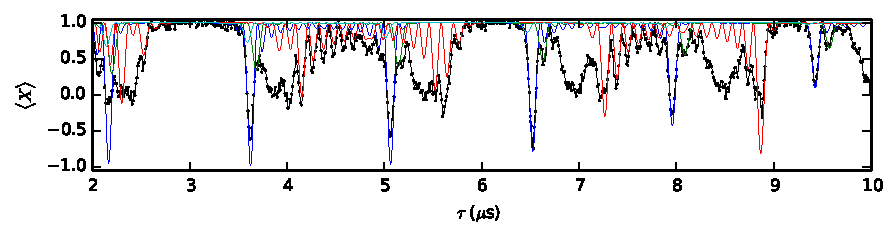
\includegraphics{Img/fingerprint16.pdf}};
            \node[font=\small, text = blue] at (4.05,1.7)  {1};
            \node[font=\small, text = green] at (9.3,2.9) {2};
            \node[font=\small, text = red] at (5.3,2.5) {3};
            \node[font=\small, text = cyan] at (4.0,3.35) {4};
            \node[font=\small, text = black] at (14.0,4.0) {$N=16$};
            % \draw[help lines,xstep=1,ystep=1] (0,0) grid (10,3);
            % \foreach \x in {1,2,...,10} { \node [anchor=north] at (\x,0) {\x}; }
            % \foreach \y in {1,2,...,3} { \node [anchor=east] at (0,\y) {\y}; }
        \end{tikzpicture}
        \label{fig:FP16}
    \end{subfigure}

    \begin{subfigure}[t]{\textwidth}\centering

    \caption{}
    \begin{tikzpicture}
        \node[anchor=south west,inner sep=0] at (0,0) {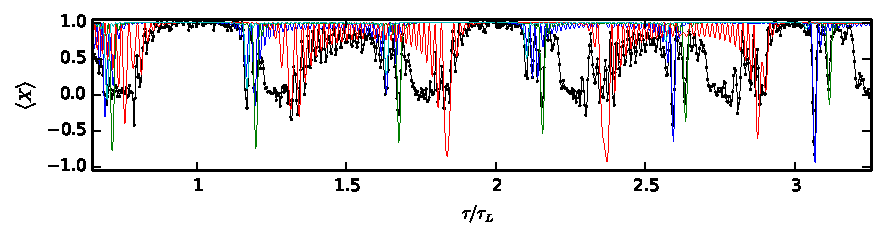
\includegraphics{Img/fingerprint32.pdf}};
        \node[font=\small, text = blue] at (11.2,1.9) {1};
        \node[font=\small, text = blue] at (4.0,2.8)  {1};
        \node[font=\small, text = green] at (6.6,1.8) {2};
        \node[font=\small, text = red] at (7.4,1.8) {3};
        \node[font=\small, text = cyan] at (4.05,2.5) {4};
        \node[font=\small, text = black] at (14.0,4.0) {$N=32$};
        % \draw[help lines,xstep=1,ystep=1] (0,0) grid (10,3);
        % \foreach \x in {1,2,...,10} { \node [anchor=north] at (\x,0) {\x}; }
        % \foreach \y in {1,2,...,3} { \node [anchor=east] at (0,\y) {\y}; }
    \end{tikzpicture}
    \label{fig:FP32}
    \end{subfigure}
    \caption{Part of a dynamical decoupling spectroscopy experiment performed at $B_z = 304\,\mathrm{G}$, $\tau_L =3.07 \, \mu \mathrm{s} $.
    Black lines correspond to data. Colored lines represent computed responses of carbon spins.
    \subref{fig:FP16} $N = 16$ pulses; \subref{fig:FP32} $N=32$ pulses.
    Contrast is lowered when the decoupling sequence performs an entangling operation on a spin in the environment.
    A reference to the full dynamical decoupling dataset can be found in \cref{chap:Fingerprint_data_appendix}.
    Responses were calculated using \cref{eq:contrast_single_carbon_spin} with hyperfine parameters from \cref{tbl:HF_par}. }
    \label{fig:FP}
\end{figure}



% Although dynamical decoupling improves the coherence of the central spin by decoupling from the environment, the central spin is also decoupled from other spins preventing direct two-qubit gates. It was demonstrated by \citet{Sar2012DecoherenceProtected} how to incorporate dynamical decoupling in a universal gate design by implementing Grover's algorithm.
% Using this technique \citet{Taminiau2012Detection} used the extended coherence to detect and control weakly-coupled carbon spins, before implementing three-qubit quantum-error-correction (QEC) \citep{Taminiau2014Universal}.

% As these experiments where performed with NV-centers at Room temperature they lack the option to do single-shot readout required to act on a measurement outcome\footnote{@Tim, I think this can be worded more concisely. Do you have any ideas?}. An essential feature for the parity measurements that form the basis of measurement-based QEC and surface codes.

% As we cannot perform an ESR experiment while decoupling a different technique must be used to resolve and address additional spins.
% In order to resolve additional spins we perform a dynamical decoupling spectroscopy, resulting in a fingerprint of the nuclear-spin environment\citep{Taminiau2012Detection}.
